\documentclass[10pt,a4paper]{report}
\usepackage[hmargin=2cm,vmargin=3.5cm,bmargin=2cm]{geometry}
\usepackage[utf8]{inputenc}
\usepackage[portuguese]{babel}
\usepackage[T1]{fontenc}
\usepackage{amsmath}
\usepackage{amsfonts}
\usepackage{amssymb}
\usepackage{makeidx}
\usepackage{graphicx}
\usepackage{listings}
\usepackage{indentfirst}
\usepackage[pdftex]{hyperref}
\usepackage{csvsimple}
\usepackage{color}

% Headers and Footers
\usepackage{fancyhdr}

\definecolor{mygreen}{rgb}{0,0.6,0}
\definecolor{mygray}{rgb}{0.5,0.5,0.5}
\definecolor{mymauve}{rgb}{0.58,0,0.82}

\lstset{ %
  backgroundcolor=\color{white},   % choose the background color; you must add \usepackage{color} or \usepackage{xcolor}
  basicstyle=\footnotesize,        % the size of the fonts that are used for the code
  breakatwhitespace=false,         % sets if automatic breaks should only happen at whitespace
  breaklines=true,                 % sets automatic line breaking
  captionpos=b,                    % sets the caption-position to bottom
  commentstyle=\color{mygreen},    % comment style
  deletekeywords={...},            % if you want to delete keywords from the given language
  escapeinside={\%*}{*)},          % if you want to add LaTeX within your code
  extendedchars=true,              % lets you use non-ASCII characters; for 8-bits encodings only, does not work with UTF-8
  frame=single,                    % adds a frame around the code
  keywordstyle=\color{blue},       % keyword style
%  language=Octave,                 % the language of the code
  morekeywords={*,...},            % if you want to add more keywords to the set
  numbers=left,                    % where to put the line-numbers; possible values are (none, left, right)
  numbersep=5pt,                   % how far the line-numbers are from the code
  numberstyle=\tiny\color{mygray}, % the style that is used for the line-numbers
  rulecolor=\color{black},         % if not set, the frame-color may be changed on line-breaks within not-black text (e.g. comments (green here))
  showspaces=false,                % show spaces everywhere adding particular underscores; it overrides 'showstringspaces'
  showstringspaces=false,          % underline spaces within strings only
  showtabs=false,                  % show tabs within strings adding particular underscores
  stepnumber=2,                    % the step between two line-numbers. If it's 1, each line will be numbered
  stringstyle=\color{mymauve},     % string literal style
  tabsize=2,                       % sets default tabsize to 2 spaces
  title=\lstname                   % show the filename of files included with \lstinputlisting; also try caption instead of title
}

% Headers and Footers
\pagestyle{fancy} % fancy style
\lhead{\rightmark} % left header
\chead{\textbf{Network Programming}} % central header
\rhead{\leftmark} % right header
\lfoot{} % left footer
\cfoot{\textbf{\thepage}} % central footer
\rfoot{} % right footer
% Headers and Footers

\makeindex

% define the title
\author{André Nakagaki Fillettaz RA: 104595 \\ Guilherme Alcarde Gallo RA: 105008}
\title{MC823 - Relat\'orio - Servidor Interativo sobre UDP}
\begin{document}

% generates the title
\maketitle

% insert the table of contents
\tableofcontents



\chapter{UDP x TCP}

	Antes de entrar em explicações e códigos do projeto client-server UDP implementado, convém uma análise prévia de algumas diferenças entre os dois protocolos, e as decisões de projeto tomadas em função dessas diferenças.

	O UDP é um protocolo de transporte livre de conexão, o que já difere do TCP. Como não há nenhum tipo de orientação a conexão (apesar da função connect() ainda estar disponível para este tipo de protocolo), o servidor UDP não utiliza processos filhos para tratar do envio de dados. Existe apenas um processo que é responsável tanto pelo tratamento da requisição quanto do envio de dados.
	
	Outra diferença decorrente disso é o envio, baseado em datagramas ao invés de stream. Isso altera em grande parte a composição do socket, e da chamada da função socket(), conforme á visto nos códigos.
	
	Por fim, já que o client e o servidor nunca estão de fato conectados, as funções de envio e recepção de dados devem ser mudadas para \textit{sendto} e \textit{recvfrom}. A diferença fundamental destas é que como não existe conexão, elas exigem por parâmetro os dados do endereço (tipo e tamanho). Isso é razoável e na vardade torna muito difícil de garantir que haverá comunicação entre os processos client-server, sendo possível executar o client por exemplo sem o server estar aberto (ocasionando obviamente erros e bugs).
	
	O UDP não é confiável, ou seja, não há garantia de entrega de datagramas, o que exige que a aplicação implemente essa “confiabilidade".
	
	Esse comportamento não confiável e não orientado à conexão torna o protocólo UDP no geral mais rápido do que o TCP, que checa a ordem de envio e procura por erros, conforme é visto na análise de dados.

\chapter{Servidor}

Processo responsável por tratar do banco de dados, tratar requisições e enviar dados ao client.

	Para tratar do banco de dados, novamente foi utilizada a biblioteca do C, SQLite3. Conforme explicado no relatório do projeto 01. Não houveram grandes mudanças nessa parte do projeto, e as funções que realizam a chamada ao banco continuam as mesmas.
	
\section{Operações}
\begin{center}
 Cada operação é representada por um inteiro no servidor: \\
\begin{tabular}{|c|c|}
\hline 
1 & Listar ISBN e Título de todos os livros \\ 
\hline 
2 & Dado o ISBN de um livro, retornar sua descrição \\ 
\hline 
3 & Dado o ISBN de um livro, retornar todas as suas informações \\ 
\hline 
4 & Listar todas as informações de todos os livros  \\ 
\hline 
5 & Atualiza estoque, caso seja cliente livraria \\ 
\hline 
6 & Dado o ISBN de um livro, retorna seu estoque \\ 
\hline
7 & Dado a senha correta, é iniciada a seção do cliente livraria \\ 
\hline
\end{tabular}
 \end{center} 
\subsection{Listagem Geral}
Aquitratam-se as operações de listagem geral. Dentre elas destacam-se entao as operações (1) e (4).

	A ideia aqui utiliza a biblioteca do SQLite3 e através de querys consulta-se o banco. Convém notar que nesse caso, a única real computação que é deixada para a função main é realizar a computação de tempo, conforme explicado a parte.
	
	A própria resposta da Query é então enviada ao client. Como exemplo, a operação (1) que lista todos os ISBNs e seus respectivos livros na biblioteca:

\begin{lstlisting}[language=C]
case 1:		// Lista de ISBN e titulo dos livros
				elapsed = 0;
				// Enviando tuplas de ISBN e titulo de todos os livros
				rc = sqlite3_exec(db, "select ISBN10,titulo from livro;", callback,
						0, &zErrMsg);
				// Tempo percorrido ate agora
				gettimeofday(&t1, 0);
				if (rc != SQLITE_OK) {
					sqlite3_free(zErrMsg);
				}

				// Finalizando a mensagem
				// Calculo do tempo de operacao
				elapsed = (t1.tv_sec - t0.tv_sec) * 1000000 + t1.tv_usec
					- t0.tv_usec;
				// Transformando em string com caracteres de "seguranca" para postumo atoi
				sprintf(query, "          %6li#", elapsed);	// Caractere # e um identificador de fim da mensagem
				// DEBUG
				printf("\nOperation Time: %s\n\n", query);
				// Calculando o tamanho
				length = strlen(query);
				// Finalmente envia para o cliente
				//					sendall(client_sock, query, &length);
				if ((numbytes = sendto(sockfd, query, strlen(query), 0,	(struct sockaddr *) &their_addr, addr_len)) == -1) {
					perror("server: sendto");
					exit(1);
				}
				break;
\end{lstlisting}

\subsection{Listagem Específica}
Aqui explica-se o funcionamento do segundo tipo de operação, as listagem específicas.

	Ao contrário da geral, nesse caso, o client deve enviar ao servidor mais do que simplesmente o número da operação solicitada, já que, nesses tipos de operações, também é necessario o número ISBN. Desse forma, são necessarios duas operações de envio por parte do client. Além disso, é necessario mais do que simplesmente realizar a query, verificar se o ISBN realmente consta no Banco de Dados.
	
	Para exemplicar esse processo de checagem e envio, o código da operação (3), listagem de informações:

\begin{lstlisting}[language=C]
case 3:
				elapsed = 0;
				// Esperando o cliente mandar o ISBN desejado
				// Tempo percorrido ate agora
				gettimeofday(&t1, 0);
				// ReCalculo do tempo de operacao
				elapsed += (t1.tv_sec - t0.tv_sec) * 1000000 + t1.tv_usec
					- t0.tv_usec;
				// Esperando o cliente mandar o ISBN desejado
				if ((read_size = recvfrom(sockfd, client_message, 2000, 0,
								(struct sockaddr *) &their_addr, &addr_len)) == -1) {
				}
				gettimeofday(&t0, 0);
				// Montando a query

				strcpy(query,
						"select l.ISBN10, l.titulo, a.autor, a.autor2, a.autor3, a.autor4, l.descricao, l.editora, l.ano, l.estoque from livro l, autor a where l.autores=a.a_id and ISBN10 = ");
				strcpy(query2, "select count(*) from livro where ISBN10 = ");
				// Concatenando o ISBN
				strcat(query, client_message);
				strcat(query2, client_message);
				// Fim do comando SQLite
				strcat(query, ";");

				// Verificando se ha livros
				// callbackSilent nao envia dados ao cliente
				// existe recebe o resultado de contagem de livros (0 ou 1)
				rc = sqlite3_exec(db, query2, callbackSilent, existe, &zErrMsg);
				if (*((int *) existe) == 0) {
					length = 41;
					//		sendall(client_sock, "\nEste ISBN nao consta na nossa livraria!\n",&length);
					gettimeofday(&t1, 0);
					if ((numbytes = sendto(sockfd,
									"\nEste ISBN nao consta na nossa livraria!\n", 42,
									0, (struct sockaddr *) &their_addr, addr_len))
							== -1) {
						perror("server: sendto");
						exit(1);
					}
					// Tempo percorrido ate agora
				} else {
					// Executando query - Callback ja faz os sends
					rc = sqlite3_exec(db, query, callbackFmt, 0, &zErrMsg);
					// Tempo percorrido ate agora
					gettimeofday(&t1, 0);
				}

				// Fim da mensagem
				// ReCalculo do tempo de operacao
				elapsed += (t1.tv_sec - t0.tv_sec) * 1000000 + t1.tv_usec
					- t0.tv_usec;
				// Transformando em string com chars de "seguranca" para postumo atoi
				sprintf(query, "          %6li#", elapsed);
				// DEBUG
				printf("\nOperation Time: %s\n\n", query);
				// Calculando o tamanho
				length = strlen(query);
				// Finalmente envia para o cliente
				//sendall(client_sock, query, &length);
				if ((numbytes = sendto(sockfd, query, strlen(query), 0,
								(struct sockaddr *) &their_addr, addr_len)) == -1) {
					perror("server: sendto");
					exit(1);
				}
				break;
\end{lstlisting}

\newpage
\subsection{Autenticação do Cliente Livraria e Mudança no estoque}


Considera-se aqui que o client normal não tem acesso a operação de mudança de estoque, apesar de poder verificar a quantidade de livros em estoque (dado um determinado ISBN).

	Caso o cliente queira mudar para o modo Livraria (Superuser) o que ele deve fazer é requisitar essa mudança e então enviar o password, que é definido no processo servidor. Aqui poderiamos expandir ainda mais o conceito, e desenvolver livrarias com bancos de dados específicos e para tanto, colocar a senha do user livraria no próprio banco de dados.

\section{Contando o tempo}


O tempo de comunicação é contado a partir do \textit{sendall} dos callbacks, pela correção no tempo gasto pelas operações feitas no próprio servidor, para que o cliente tenha informações corretas do tempo gasto somente na comunicação, e pelo respectivo \textit{receive} acionado pelo cliente.

Para contar o tempo, utilizou-se a função \textit{gettimeofday} e duas variáveis do tipo \textit{struct timeval}, ambos da biblioteca \textbf{time.h}.

A contagem de tempo funciona como uma sequencia de cronometragens. No servidor, estas ignoram o tempo gasto com \emph{receives} e contam apenas o tempo das \emph{operações}, já -- no cliente -- a sequencia de cronometragens é cautelosa para apenas medir o tempo dos \emph{receives}.

A ideia de cronometragem vem de uma subtração de tempo $final - inicial$, calculado em milisegundos, pela fórmula dada pela equação:
\begin{equation}
elapsed += (t_{final}.tv\_sec-t_{inicial}.tv\_sec)*1000000 + t_{final}.tv\_usec-t_{inicial}.tv\_usec;
\end{equation}

Para exemplificar, o código da operação 2:

\begin{lstlisting}[language=C]
case 2:		// Descricao de um livro
				elapsed = 0;
				// Esperando o cliente mandar o ISBN desejado
				// Tempo percorrido ate agora
				gettimeofday(&t1, 0);
				// ReCalculo do tempo de operacao
				elapsed += (t1.tv_sec - t0.tv_sec) * 1000000 + t1.tv_usec
					- t0.tv_usec;

				printf("\nISBN1:%s\n", client_message);
				if ((numbytes = recvfrom(sockfd, client_message, MAXBUFLEN - 1, 0,
								(struct sockaddr *) &their_addr, &addr_len)) == -1) {
					perror("recvfrom");
					exit(1);
				}
				gettimeofday(&t0, 0);
				// Montando a query
				strcpy(query, "select descricao from livro where ISBN10 = ");
				strcpy(query2,
						"select count(descricao) from livro where ISBN10 = ");
				printf("\nISBN2:%s\n", client_message);
				// Concatenando o ISBN
				strcat(query, client_message);
				strcat(query2, client_message);
				// Fim do comando SQLite
				strcat(query, ";");

				// Verificando se ha livros
				// callbackSilent nao envia dados ao cliente
				// existe recebe o resultado de contagem de livros (0 ou 1)
				rc = sqlite3_exec(db, query2, callbackSilent, existe, &zErrMsg);
				// Tempo percorrido ate agora
				//	gettimeofday(&t1, 0);
				if (*((int *) existe) == 0) {
					//				sendall(client_sock, "\nEste ISBN nao consta na nossa livraria!\n",&length);
					if ((numbytes = sendto(sockfd,
									"\nEste ISBN nao consta na nossa livraria!\n", 42,
									0, (struct sockaddr *) &their_addr, addr_len))
							== -1) {
						perror("server: sendto");
						exit(1);
					}
				} else
					// Executando query - Callback ja faz os sends
					rc = sqlite3_exec(db, query, callback, 0, &zErrMsg);
				gettimeofday(&t1, 0);
				// Fim da mensagem
				// ReCalculo do tempo de operacao
				elapsed += (t1.tv_sec - t0.tv_sec) * 1000000 + t1.tv_usec
					- t0.tv_usec;
				// Transformando em string com chars de "seguranca" para postumo atoi
				sprintf(query, "          %6li#", elapsed);
				// DEBUG
				printf("\nOperation Time: %s\n\n", query);
				// Calculando o tamanho
				length = strlen(query);
				// Finalmente envia para o cliente
				//sendall(client_sock, query, &length);
				if ((numbytes = sendto(sockfd, query, strlen(query), 0,
								(struct sockaddr *) &their_addr, addr_len)) == -1) {
					perror("server: sendto");
					exit(1);
				}
				break;
\end{lstlisting}

\section{Código Completo}
Assim como no TCP, o servidor UDP foi fortemente baseado no Beej's Guide to Network Programming.
\begin{lstlisting}[language=C,label=callback]
/*
 ** listener.c -- a datagram sockets "server" demo
 */

#include <stdio.h>
#include <stdlib.h>
#include <unistd.h>
#include <errno.h>
#include <string.h>
#include <sys/types.h>
#include <sys/socket.h>
#include <netinet/in.h>
#include <arpa/inet.h>
#include <netdb.h>

#define MYPORT "4950"	// the port users will be connecting to
#define MAXBUFLEN 100

// SQLite3
#include <sqlite3.h>

#define PASSWORD "numaPistacheCottapie"
int sockfd;
struct sockaddr_storage their_addr;
socklen_t addr_len;
int numbytes;

typedef struct livro {
	char i[20];	// ISBN
	char q[4];	// Stock Quantity
} Livro;

int socket_desc, client_sock, c, read_size, connfd;

// Tempo
long elapsed = 0;			// Conta o tempo percorrido
struct timeval t0, t1;

// get sockaddr, IPv4 or IPv6:
void *get_in_addr(struct sockaddr *sa) {
	if (sa->sa_family == AF_INET) {
		return &(((struct sockaddr_in*) sa)->sin_addr);
	}

	return &(((struct sockaddr_in6*) sa)->sin6_addr);
}

// Callback do SQLite3. Versao silenciosa, nao envia nada para o cliente
static int callbackSilent(void *NotUsed, int argc, char **ans,
		char **azColName) {
	int i, num;
	int *v;
	v = (int *) alloca(sizeof(int));
	// Aaaaaaah Moleque!!!!!
	v = NotUsed;
	*v = atoi(ans[0]);
	//	printf("\n--------\n%d\n--------\n",*v);
	return 0;
}

// Callback do SQLite3. Versao formatada para varios detalhes
static int callbackFmt(void *NotUsed, int argc, char **ans, char **azColName) {
	int i, num;
	char aux[20000];

	// Nome da coluna
	strcpy(aux, azColName[0]);
	strcat(aux, ": ");
	// Concatena valor
	strcat(aux, ans[0]);
	strcat(aux, "\n");
	// Formata
	for (i = 1; i < argc; i++) {		// Fazendo isso para o resto da tupla
		if (ans[i]) {
			strcat(aux, azColName[i]);
			strcat(aux, ": ");
			// Melhorando a visualizacao da descricao
			if (i == 3) {
				strcat(aux, "\n\t");
			}
			strcat(aux, ans[i]);
			strcat(aux, "\n");
		}
	}
	strcat(aux, "\n");
	// DEBUG
	printf("%s", aux);
	// Enviando para o cliente
	num = strlen(aux);
	gettimeofday(&t1, 0);
	elapsed += (t1.tv_sec-t0.tv_sec)*1000000 + t1.tv_usec-t0.tv_usec;
	if ((numbytes = sendto(sockfd, aux, strlen(aux), 0,
					(struct sockaddr *) &their_addr, addr_len)) == -1) {
		perror("server: sendto");
		exit(1);
	}
	gettimeofday(&t0, 0);
	return 0;
}

// Callback formatado em tupla simples
static int callback(void *NotUsed, int argc, char **ans, char **azColName) {
	int i, num;
	char aux[20000];

	strcpy(aux, ans[0]);
	for (i = 0; i < argc; i++) {
		if (i && ans[i]) {
			strcat(aux, " | ");
			strcat(aux, ans[i]);
		}
	}
	strcat(aux, "\n");
	printf("Tamanho= %d\n%s", (int)strlen(aux), aux);
	num = strlen(aux);
	gettimeofday(&t1, 0);
	elapsed += (t1.tv_sec-t0.tv_sec)*1000000 + t1.tv_usec-t0.tv_usec;
	if ((numbytes = sendto(sockfd, aux, strlen(aux), 0,
					(struct sockaddr *) &their_addr, addr_len)) == -1) {
		perror("server: sendto");
		exit(1);
	}
	gettimeofday(&t0, 0);
	return 0;
}

int main(void) {
	struct addrinfo hints, *servinfo, *p;
	int rv;
	char buf[MAXBUFLEN];
	char s[INET6_ADDRSTRLEN];


	char client_message[2000], query[2500], query2[2500];

	int opcao;

	// SQLite3
	sqlite3 *db;
	char *zErrMsg = 0, *msg;
	int rc;
	void *existe; 				// Para requisicoes invalidas
	int superuser = 0; 			// Cliente Livraria
	existe = (void *) alloca(sizeof(int));	// Usado para saber se o ISBN existe
	Livro cm;

	// Timeout setado para imprevistos ...
	struct timeval tv;

	tv.tv_sec = 5; /* 30 Secs Timeout */
	tv.tv_usec = 0;  // Not init'ing this can cause strange errors

	setsockopt(connfd, SOL_SOCKET, SO_RCVTIMEO, (char *) &tv,
			sizeof(struct timeval));
	// ... Timeout setado.

	// Abrindo Banco de Dados do SQLite3
	rc = sqlite3_open("livraria2.db", &db);

	memset(&hints, 0, sizeof hints);
	hints.ai_family = AF_UNSPEC; // set to AF_INET to force IPv4
	hints.ai_socktype = SOCK_DGRAM;
	hints.ai_flags = AI_PASSIVE; // use my IP

	// Servidor interativo
	while (1) {
		if ((rv = getaddrinfo(NULL, MYPORT, &hints, &servinfo)) != 0) {
			fprintf(stderr, "getaddrinfo: %s\n", gai_strerror(rv));
			return 1;
		}

		// loop through all the results and bind to the first we can
		for (p = servinfo; p != NULL; p = p->ai_next) {
			if ((sockfd = socket(p->ai_family, p->ai_socktype, p->ai_protocol))
					== -1) {
				perror("listener: socket");
				continue;
			}

			if (bind(sockfd, p->ai_addr, p->ai_addrlen) == -1) {
				close(sockfd);
				perror("listener: bind");
				continue;
			}

			break;
		}

		if (p == NULL) {
			fprintf(stderr, "listener: failed to bind socket\n");
			return 2;
		}

		freeaddrinfo(servinfo);

		printf("listener: waiting to recvfrom...\n");

		addr_len = sizeof their_addr;
		if ((numbytes = recvfrom(sockfd, buf, MAXBUFLEN - 1, 0,
						(struct sockaddr *) &their_addr, &addr_len)) == -1) {
			perror("recvfrom");
			exit(1);
		}
		// Comecando a contar o tempo de operacao
		gettimeofday(&t0, 0);

		printf("listener: got packet from %s\n",
				inet_ntop(their_addr.ss_family,
					get_in_addr((struct sockaddr *) &their_addr), s,
					sizeof s));

		printf("listener: packet is %d bytes long\n", numbytes);
		buf[numbytes] = '\0';
		printf("listener: packet contains \"%s\"\n", buf);

		opcao = atoi(buf);

		switch (opcao) {
			case 1:		// Lista de ISBN e titulo dos livros
				elapsed = 0;
				// Enviando tuplas de ISBN e titulo de todos os livros
				rc = sqlite3_exec(db, "select ISBN10,titulo from livro;", callback,
						0, &zErrMsg);
				// Tempo percorrido ate agora
				gettimeofday(&t1, 0);
				if (rc != SQLITE_OK) {
					sqlite3_free(zErrMsg);
				}

				// Finalizando a mensagem
				// Calculo do tempo de operacao
				elapsed = (t1.tv_sec - t0.tv_sec) * 1000000 + t1.tv_usec
					- t0.tv_usec;
				// Transformando em string com caracteres de "seguranca" para postumo atoi
				sprintf(query, "          %6li^D", elapsed);	// Caractere ^D e um identificador de fim da mensagem
				// DEBUG
				printf("\nOperation Time: %s\n\n", query);
				// Calculando o tamanho
				// Finalmente envia para o cliente
				if ((numbytes = sendto(sockfd, query, strlen(query), 0,	(struct sockaddr *) &their_addr, addr_len)) == -1) {
					perror("server: sendto");
					exit(1);
				}
				break;

				/***********************************/

			case 2:		// Descricao de um livro
				elapsed = 0;
				// Esperando o cliente mandar o ISBN desejado
				// Tempo percorrido ate agora
				gettimeofday(&t1, 0);
				// ReCalculo do tempo de operacao
				elapsed += (t1.tv_sec - t0.tv_sec) * 1000000 + t1.tv_usec
					- t0.tv_usec;

				printf("\nISBN1:%s\n", client_message);
				if ((numbytes = recvfrom(sockfd, client_message, MAXBUFLEN - 1, 0,
								(struct sockaddr *) &their_addr, &addr_len)) == -1) {
					perror("recvfrom");
					exit(1);
				}
				gettimeofday(&t0, 0);
				// Montando a query
				strcpy(query, "select descricao from livro where ISBN10 = ");
				strcpy(query2,
						"select count(descricao) from livro where ISBN10 = ");
				printf("\nISBN2:%s\n", client_message);
				// Concatenando o ISBN
				strcat(query, client_message);
				strcat(query2, client_message);
				// Fim do comando SQLite
				strcat(query, ";");

				// Verificando se ha livros
				// callbackSilent nao envia dados ao cliente
				// existe recebe o resultado de contagem de livros (0 ou 1)
				rc = sqlite3_exec(db, query2, callbackSilent, existe, &zErrMsg);
				// Tempo percorrido ate agora
				//	gettimeofday(&t1, 0);
				if (*((int *) existe) == 0) {
					if ((numbytes = sendto(sockfd,
									"\nEste ISBN nao consta na nossa livraria!\n", 42,
									0, (struct sockaddr *) &their_addr, addr_len))
							== -1) {
						perror("server: sendto");
						exit(1);
					}
				} else
					// Executando query - Callback ja faz os sends
					rc = sqlite3_exec(db, query, callback, 0, &zErrMsg);
				gettimeofday(&t1, 0);
				// Fim da mensagem
				// ReCalculo do tempo de operacao
				elapsed += (t1.tv_sec - t0.tv_sec) * 1000000 + t1.tv_usec
					- t0.tv_usec;
				// Transformando em string com chars de "seguranca" para postumo atoi
				sprintf(query, "          %6li^D", elapsed);
				// DEBUG
				printf("\nOperation Time: %s\n\n", query);
				// Calculando o tamanho
				// Finalmente envia para o cliente
				if ((numbytes = sendto(sockfd, query, strlen(query), 0,
								(struct sockaddr *) &their_addr, addr_len)) == -1) {
					perror("server: sendto");
					exit(1);
				}
				break;

				/***********************************************/


			case 3:		// Todas as informacoes de um livro
				elapsed = 0;
				// Esperando o cliente mandar o ISBN desejado
				// Tempo percorrido ate agora
				gettimeofday(&t1, 0);
				// ReCalculo do tempo de operacao
				elapsed += (t1.tv_sec - t0.tv_sec) * 1000000 + t1.tv_usec
					- t0.tv_usec;
				// Esperando o cliente mandar o ISBN desejado
				if ((read_size = recvfrom(sockfd, client_message, 2000, 0,
								(struct sockaddr *) &their_addr, &addr_len)) == -1) {
				}
				gettimeofday(&t0, 0);
				// Montando a query

				strcpy(query,
						"select l.ISBN10, l.titulo, a.autor, a.autor2, a.autor3, a.autor4, l.descricao, l.editora, l.ano, l.estoque from livro l, autor a where l.autores=a.a_id and ISBN10 = ");
				strcpy(query2, "select count(*) from livro where ISBN10 = ");
				// Concatenando o ISBN
				strcat(query, client_message);
				strcat(query2, client_message);
				// Fim do comando SQLite
				strcat(query, ";");

				// Verificando se ha livros
				// callbackSilent nao envia dados ao cliente
				// existe recebe o resultado de contagem de livros (0 ou 1)
				rc = sqlite3_exec(db, query2, callbackSilent, existe, &zErrMsg);
				if (*((int *) existe) == 0) {
					gettimeofday(&t1, 0);
					if ((numbytes = sendto(sockfd,
									"\nEste ISBN nao consta na nossa livraria!\n", 42,
									0, (struct sockaddr *) &their_addr, addr_len))
							== -1) {
						perror("server: sendto");
						exit(1);
					}
					// Tempo percorrido ate agora
				} else {
					// Executando query - Callback ja faz os sends
					rc = sqlite3_exec(db, query, callbackFmt, 0, &zErrMsg);
					// Tempo percorrido ate agora
					gettimeofday(&t1, 0);
				}

				// Fim da mensagem
				// ReCalculo do tempo de operacao
				elapsed += (t1.tv_sec - t0.tv_sec) * 1000000 + t1.tv_usec
					- t0.tv_usec;
				// Transformando em string com chars de "seguranca" para postumo atoi
				sprintf(query, "          %6li^D", elapsed);
				// DEBUG
				printf("\nOperation Time: %s\n\n", query);
				// Calculando o tamanho
				// Finalmente envia para o cliente
				if ((numbytes = sendto(sockfd, query, strlen(query), 0,
								(struct sockaddr *) &their_addr, addr_len)) == -1) {
					perror("server: sendto");
					exit(1);
				}
				break;

			case 4:		// Todas as informacoes de todos os livros
				elapsed = 0;
				// Executando query
				rc =
					sqlite3_exec(db,
							"select l.ISBN10, l.titulo, a.autor, a.autor2, a.autor3, a.autor4, l.descricao, l.editora, l.ano, l.estoque from livro l, autor a where l.autores=a.a_id;",
							callbackFmt, 0, &zErrMsg);

				// Fim da mensagem
				// Tempo percorrido ate agora
				gettimeofday(&t1, 0);
				// Calculo do tempo de operacao
				elapsed = (t1.tv_sec - t0.tv_sec) * 1000000 + t1.tv_usec
					- t0.tv_usec;
				// Transformando em string com chars de "seguranca" para postumo atoi
				sprintf(query, "          %6li^D", elapsed);
				// DEBUG
				printf("\nOperation Time: %s\n\n", query);
				// Calculando o tamanho
				// Finalmente envia para o cliente
				if ((numbytes = sendto(sockfd, query, strlen(query), 0,
								(struct sockaddr *) &their_addr, addr_len)) == -1) {
					perror("server: sendto");
					exit(1);
				}

				break;

				/*******************************************/

			case 5:		// Atualizar estoque
				elapsed = 0;
				// Tempo percorrido ate agora
				gettimeofday(&t1, 0);
				// ReCalculo do tempo de operacao
				elapsed += (t1.tv_sec - t0.tv_sec) * 1000000 + t1.tv_usec
					- t0.tv_usec;
				if ((read_size = recvfrom(sockfd, &cm, 2000, 0,
								(struct sockaddr *) &their_addr, &addr_len)) == -1) {
					perror("server: sendto");
					exit(1);
				}
				gettimeofday(&t0, 0);
				if (superuser) {
					// Montando a query
					strcpy(query, "update livro set estoque = ");
					// Concatenando o nova quantidade do estoque
					strcat(query, cm.q);
					// Concatenando o ISBN
					strcat(query, " where ISBN10 = ");
					strcat(query, cm.i);
					// Fim do comando SQLite
					strcat(query, ";");
					printf("%s\n", query);
					// Executando query - Callback ja faz os writes
					rc = sqlite3_exec(db, query, callback, 0, &zErrMsg);
				} else {
					if ((numbytes = sendto(sockfd, "Sem permissoes para modificar estoque!\n", 42, 0,
									(struct sockaddr *) &their_addr, addr_len)) == -1) {
						perror("server: sendto");
						exit(1);
					}

				}

				// Fim da mensagem
				// Tempo percorrido ate agora
				gettimeofday(&t1, 0);
				// ReCalculo do tempo de operacao
				elapsed += (t1.tv_sec - t0.tv_sec) * 1000000 + t1.tv_usec
					- t0.tv_usec;
				// Transformando em string com chars de "seguranca" para postumo atoi
				sprintf(query, "          %6li^D", elapsed);
				// DEBUG
				printf("\nTime: %s\n\n", query);
				// Calculando o tamanho
				// Finalmente envia para o cliente
				if ((numbytes = sendto(sockfd, query, strlen(query), 0,
								(struct sockaddr *) &their_addr, addr_len)) == -1) {
					perror("server: sendto");
					exit(1);
				}

				break;

			case 6:		// Mostra estoque de um livro
				elapsed = 0;
				// Tempo percorrido ate agora
				gettimeofday(&t1, 0);
				// ReCalculo do tempo de operacao
				elapsed += (t1.tv_sec-t0.tv_sec)*1000000 + t1.tv_usec-t0.tv_usec;
				// Esperando o cliente mandar o ISBN desejado
				if ((numbytes = recvfrom(sockfd, client_message, MAXBUFLEN - 1, 0,
								(struct sockaddr *) &their_addr, &addr_len)) == -1) {
					perror("recvfrom");
					exit(1);
				}
				gettimeofday(&t0, 0);
				// Montando a query
				strcpy(query, "select estoque from livro where ISBN10 = ");
				// Concatenando o ISBN
				strcat(query, client_message);
				// Fim do comando SQLite
				strcat(query, ";");
				printf("\n%s\n", query);
				// Executando query - Callback ja faz os writes
				rc = sqlite3_exec(db, query, callbackFmt, 0, &zErrMsg);
				// Fim da mensagem
				// Tempo percorrido ate agora
				gettimeofday(&t1, 0);
				// ReCalculo do tempo de operacao
				elapsed += (t1.tv_sec-t0.tv_sec)*1000000 + t1.tv_usec-t0.tv_usec;
				// Transformando em string com chars de "seguranca" para postumo atoi
				sprintf(query,"          %6li^D",elapsed);
				// DEBUG
				printf("\nTime: %s\n\n",query);
				// Calculando o tamanho
				// Finalmente envia para o cliente
				if ((numbytes = sendto(sockfd, query, strlen(query), 0,
								(struct sockaddr *) &their_addr, addr_len)) == -1) {
					perror("server: sendto");
					exit(1);
				}
				break;
			case 7:		// Autentica o cliente livraria
				// Recebe a senha
				if ((numbytes = recvfrom(sockfd, client_message, 50, 0,
								(struct sockaddr *) &their_addr, &addr_len)) == -1) {
					perror("recvfrom");
					exit(1);
				}
					// Compara as senhas
					if( (strcmp(client_message,PASSWORD) ) == 0) {
						superuser = 1;		// Sessao de superusuario
						if ((numbytes = sendto(sockfd, "Bem-vindo, Chuck Norris!\n\n", 31, 0,
										(struct sockaddr *) &their_addr, addr_len)) == -1) {
							perror("server: sendto");
							exit(1);
						}
					}
					else {
						superuser = 0;		// Usuario invalido
						if ((numbytes = sendto(sockfd, "Senha Invalida!\n\n", 18, 0,
										(struct sockaddr *) &their_addr, addr_len)) == -1) {
							perror("server: sendto");
							exit(1);
						}
					}
					memset(client_message,0,strlen(client_message));
				break;

		}
		close(sockfd);
	}
	return 0;
}
\end{lstlisting}

\chapter{Cliente}

O processo client tem por responsabilidade receber e lidar com as requisições por parte do user do sistema e fazer essas requisições para um servidor que opere em protocolo UDP.

	Inicia apresentando as opções ao usuario, e depois disso espera por uma opção de entrada. Ao receber essa opção, novamente através da função dataFetch (agora modificada para operar em protocólo UDP). Essa função trata de quase todos os tipos de operação do servidor, sendo que apenas para as funções que mexem no estoque ela não é utilizada.

\section*{Código Completo}
\begin{center}
Arquivo: Client.h
\end{center}
\begin{lstlisting}[language=C]
/* Client.c - UDP Socket ------------------------------------------------------
 * Andre Nakagaki Filliettaz 	- RA104595 --------------------------------------
 * Guilerme Alcarde Gallo 		- RA105008 --------------------------------------
 ----------------------------------------------------------------------------*/

/* This programs deals with the interface with the humans and requests to
 * to the server. Uses the standarts UDP sockets and SQLite3 librarys */

/* Include all the stuff need to execute the program */
#include "Client.h"
#define MYPORT "4950"
#define SERVIP "143.106.16.244"		// Ribeiro - IC301

/* Main function */
int main (int argc, char *argv[]) {
	/* Control Variables */
	char op, isbn[11], pwd[50], qtt[4], sIP[20];

	/* With the connection done, read to send requests to the server */
	int sockfd;
	struct addrinfo hints, *servinfo, *tmp;
	char message[1000] , server_reply[2000];
	struct timeval tv;

	tv.tv_sec = 5;  /* 30 Secs Timeout */
	tv.tv_usec = 0;  // Not init'ing this can cause strange errors


	/* Defining the IP */
	if (argv[1] == NULL)	strcpy(sIP, SERVIP);		/* Default */
	else if (argv[1]=="0")	strcpy(sIP, "127.0.0.1");	/* Host */
	else 			strcpy(sIP, argv[1]);		/* Passed */

	/* Setting hints to get the list of addrinfo struct */
	memset(&hints, 0, sizeof hints);
	hints.ai_family = AF_UNSPEC;	/* Any kind of IP */
	hints.ai_socktype = SOCK_DGRAM;	/* UDP */


	/* Create the list of structs */
	if (getaddrinfo (sIP,MYPORT, &hints, &servinfo) != 0) {
		printf("Erro na alocacao de Enderecos!\n");
		return -1;
	}

	/* Take the first of the addrinfo inside the list */
	for (tmp = servinfo; tmp != NULL; tmp = tmp->ai_next) {
		/* Get the Socket Descriptor */
		if ((sockfd = socket(tmp->ai_family, tmp->ai_socktype, tmp->ai_protocol)) == -1 ) {
			printf("Error on socket creation! Trying next address struct!\n");
			continue;
		}
		break;
	}

	if (tmp == NULL) {
		printf("Falha ao criar sockets! Abortando!\n");
		return -2;
	}


	/* Start the loop of requests to the server! */
	while(1) {
		showOptions();	// Explains the options to the User

		scanf(" %c", &op);	// Take the option from user


		switch(op) {
			case 'h':	// A little help
				break;


			case 'l':	// Looking at the Store
				if( dataFetch(sockfd, NULL, "1", tmp) < 0)
					printf("PROBLEMS!!!!!!!\n");
				break;


			case 'd':	// Searching for Description
				printf("Waiting for ISBN of the Book!\n");
				scanf(" %s", isbn);	// Getting ISBN

				/* Calling the fetching result function */
				dataFetch(sockfd, isbn, "2", tmp);
				break;


			case 'i':	// Searching for Info
				printf("Waiting for ISBN of the Book!\n");
				scanf(" %s", isbn);	// Getting ISBN

				/* Calling the fetching result function  */
				printf("%d",dataFetch(sockfd, isbn, "3", tmp));
				break;


			case 'a':	// All Infos
					/* Calling the fetching result function  */
				if( dataFetch(sockfd, NULL, "4", tmp) < 0)
					printf("PROBLEMS!!!!!!!\n");
				break;


			case 'c':	// Changing the stores numbers
				printf("Waiting for the new stock amount!\n");
				scanf(" %s", qtt);	// Getting Quantity
				printf("Waiting for ISBN of the Book!\n");
				scanf(" %s", isbn);	// Getting ISBN
				alterStock(sockfd, isbn, qtt, tmp);
				break;


			case 'n':	// Numbers on stock
				printf("Waiting for ISBN of the Book!\n");
				scanf("%s", isbn);	// Getting ISBN

				/* Calling the stocks numbers */
				dataFetch(sockfd, isbn, "6", tmp);
				break;


			case 'p':
				printf("Digite a senha para cliente livraria...\n");
				scanf(" %s", pwd);
				pass(sockfd, pwd, tmp);
				break;


			case 'q':	// Quiting the program!
				printf("Quiting now!\n");
				break;


			default:	// Unknow command
				printf("Bad instruction, try again!\n");
				break;
		} /* End Switch */

		if (op == 'q')
			break;

	}
	
	close(sockfd);
	return 0;	// Terminating program

}
\end{lstlisting}

\begin{center}
Arquivo: CliFunctions.c
\end{center}
\begin{lstlisting}[language=C]
/* CliFunctions.c - UDP Socket ------------------------------------------------
 * Andre Nakagaki Filliettaz 	- RA104595 --------------------------------------
 * Guilherme Alcarde Gallo 		- RA105008 --------------------------------------
 * -------------------------------------------------------------------------- */

/* Implementation of all the functions used on Client.c  */

/* Include all the stuff need to execute the program */
#include "Client.h"

int check_str(char str[], char alpha) {
	int it=0, count=0;

	/* Looping on the string */
	for(it=0; it < strlen(str); it++) {
		if(str[it] == alpha)	count++;

	}

	/* char didn't find */
	return count;
}

void logger(char option[], int time, int countR, int tOp) {
	FILE *logfile;
	char text[50], name[10];
	
	sprintf(name,"LOG%s", option);
	// Gravando opcao e tempo percorrido em foramto CSV
	sprintf(text,"%s,%d,%d,%d\n", option, time, countR, tOp);
	logfile = fopen(name,"a");
	fputs(text,logfile);
	fclose(logfile);
}

/* -------------------------------------------------------------------------- */

void showOptions() {
	printf("Welcome to the Library! Enter the option following the notation:\n");
	printf("[h]: Help 	  - Show this message again!\n");
	printf("[l]: List  	  - List all the ISBN and his respects Titles\n");
	printf("[d]: Description  - Show the description of a given ISBN\n");
	printf("[i]: Information  - Displays the infos from a given ISBN\n");
	printf("[a]: All Infos	  - Show all the infos from all the books\n");
	printf("[p]: Password	  - Authenticate the livraria account\n");
	printf("[c]: Changing	  - Change the numbers of the Stock **\n");
	printf("[n]: On Stock	  - Numbers on Stock\n");
	printf("[q]: Quit	  - Bye Bye!\n\n");

	printf("---------\n");
	printf("** Administrator Only!\n\n");

	printf("Make your choice: ");
}

/* -------------------------------------------------------------------------- */

void alterStock(int sockfd, char isbn[], char qtd[], struct addrinfo *saddr) {
	char asw[5000];	// Response from server
	char *time;	// Operation Time from the Server
	int read_bytes,sig=0;

	Livro tt;
	strcpy(tt.i,isbn);
	strcpy(tt.q,qtd);

	long elapsed = 0; 	// Guarda intervalo de tempo
	int nRevcs = 0;		// Guarda numero de receives
	struct timeval t0, t1;	// Guarda tempo percorrido

	// Sending request for password to server
	if ( sendto(sockfd, "5", 2, 0, saddr->ai_addr, saddr->ai_addrlen) < 0) {
		printf("SEND FAILURE!\n");	// DEBUG 
		return;
	}

	// Sending the password string to server
	if ( sendto(sockfd, &tt, 30, 0, saddr->ai_addr, saddr->ai_addrlen) < 0) {
		printf("SEND FAILURE!\n");	// DEBUG 
		return;
	}

	// Receiving the answer of server authentication
	while(1) {

		/* Cleans the string */
		memset(asw,0,5000);

		gettimeofday(&t0, 0);		// Capturando tempo de inicio
		/* Read a maximum of 500 bytes from buffer */
		if ( read_bytes = recvfrom(sockfd, asw, 5000, 0, saddr->ai_addr, &saddr->ai_addrlen) < 0 ) {
			printf("Erro no receive!!\n\n");
			return;
		} else {
			gettimeofday(&t1, 0);	// Capturando tempo de termino
			nRevcs++;		// Atualizando contagem de receive
			// Calculando intervalo de tempo em microsegundos
			elapsed += (t1.tv_sec-t0.tv_sec)*1000000 + t1.tv_usec-t0.tv_usec;
			 /* Tests if received string contains the char
			  * '^D', which means TRANSMISSION OVER */
			 sig=check_str(asw, '^D');
			 
			 /* Testing here what is what... */
			 if (sig > 0) {
				 /* End Reading */
				 printf("%s", asw);
				 break;
			 } else  /* Continue Reading! */
				 printf("%s", asw);
			 
		}
	}

	printf("%s",asw);
	time = asw+strlen(asw)-8;
	printf("\n");
	printf("Tempo gasto: %lius || %li || %li", elapsed - (long)atoi(time), elapsed, (long)atoi(time));
	printf("\n");
	logger("5",elapsed - atoi(time),nRevcs,atoi(time));
	elapsed = 0;
}

/* -------------------------------------------------------------------------- */

void pass(int sockfd, char pwd[], struct addrinfo *saddr) {
	char asw[5000];	// Response from server

	// Sending request for password to server
	if ( sendto(sockfd, "7", 2, 0, saddr->ai_addr, saddr->ai_addrlen) < 0) {
		printf("SEND FAILURE!\n");	// DEBUG 
		return;
	}

	// Sending the password string to server
	if ( sendto(sockfd, pwd, 50, 0, saddr->ai_addr, saddr->ai_addrlen) < 0) {
		printf("SEND FAILURE!\n");	// DEBUG 
		return;
	}

	// Receiving the answer of server authentication
	if ( recvfrom(sockfd, asw, 200, 0, saddr->ai_addr, &saddr->ai_addrlen) < 0 ) {
		printf("[1] RECEIVE FAILURE\nasw: %s", asw );	// DEBUG
		return;
	}

	printf("%s",asw);
}


/* -------------------------------------------------------------------------- */

int dataFetch(int sockfd, char *ISBN, char op[], struct addrinfo *saddr) {
	char asw[5000];	// Answer from the Server
	char *time;	// Operation Time from the Server
	int read_bytes, sig=0, errc=0;
	
	socklen_t addr_len;

	long elapsed = 0; 	// Guarda intervalo de tempo
	int nRevcs = 0;		// Guarda numero de receives
	struct timeval t0, t1;	// Guarda tempo percorrido

	/* Formating output */
	printf("\n");
	
	/* Sends the Request to the Server and check errors */
	if ( sendto(sockfd, op, strlen(op), 0, saddr->ai_addr, saddr->ai_addrlen) < 0 ) {
		printf("Sending Error! Aborting!\n");
		return -1;
	}

	if ( op[0] != '1' && op[0] != '4' ) {
		/* Send the ISBN required to the operation in case
		 * of operations 2 and 3 */
		if ( sendto(sockfd, ISBN, strlen(ISBN), 0, saddr->ai_addr, saddr->ai_addrlen) < 0 ) {
			printf("Sending Error! Aborting!\n");
			return -1;
		}

	}


	/* Reading L00P! Read from the buffer as long there is data at the buffer,
	 * if receives the signal to stop (char '^D') then stop reading */
	elapsed = 0;
	
	while(1) {

		/* Cleans the string */
		memset(asw,0,5000);

		gettimeofday(&t0, 0);		// Capturando tempo de inicio

		/* Read a maximum of 5000 bytes from buffer */
		if ( read_bytes = recvfrom(sockfd, asw, 5000, 0, saddr->ai_addr, &saddr->ai_addrlen) < 0 ) 
			 return -1;
		else {
			gettimeofday(&t1, 0);	// Capturando tempo de termino
			nRevcs++;		// Atualizando contagem de receive
			
			// Calculando intervalo de tempo em microsegundos
			elapsed += (t1.tv_sec-t0.tv_sec)*1000000 + t1.tv_usec-t0.tv_usec;

			/* Tests if received string contains the char
			 * '^D', which means TRANSMISSION OVER */
			sig=check_str(asw, '^D');

			/* Testing here what is what... */
			if (sig > 0) {
				/* End Reading */
				printf("%s", asw);
				break;
			} else  /* Continue Reading! */
				printf("%s", asw);

		}
	}

	/* Formating the output! */
	time = asw+strlen(asw)-8;
	printf("\n");
	printf("Tempo gasto: %lius || %li || %li -- %d", elapsed - (long)atoi(time), elapsed, (long)atoi(time), nRevcs);
	printf("\n");
	printf("%s",time);
	printf("\n");
	// Guardando num log CSV
	logger(op,elapsed-atoi(time),nRevcs,atoi(time));
	elapsed = 0;
	return 0;
	
}

/* -------------------------------------------------------------------------- */

/* -------------------------------------------------------------------------- */
\end{lstlisting}

\section{Explicações das Funções Principais}
Essas quatro primeiras rotinas foram implementadas para fazer o trabalho principal de enviar requisições ao sistema e receber dados do usuário do mesmo:
\begin{itemize}
\item \textbf{int main(int argc, char *argv[])}: é a função responsável por gerenciar as chamadas de outras funções que realizarão as requisições de dados. Uma coisa importante implementada nesta função é a criação do socket. Além disso, ela pode ou não receber parâmetros em sua chamada. Se receber “0”, utiliza como IP o do proprio host, ou seja, busca se conectar a um servidor em 127.0.0.1. Caso o primeiro argumento de sua chamada for qualquer tipo de string, essa string será interpretada como um endereço IP. Por fim, se não houverem argumentos na chamada, o endereço utilizado para fazer o envio de dados será um default, especificado no código;
\item \textbf{int dataFetch(int, char, char [], addrinfo \**)}: a função mais importante do processo Client! Recebe como parâmetros o descritor de socket,  uma string, que pode conter o ISBN do livro dependendo da opção escolhida pelo usuário, ou NULL, a tarefa que deve ser executada pelo servidor e um pointer para uma estrutura \textit{addrinfo} (cujo uso será explicado mais abaixo). É chamada multiplas vezes pela função main, por ser a rotina responsável por enviar as requisições ao servidor, bem como imprimir os resultados na tela. A impressão é feita diretamente da leitura do buffer, sendo que a função sabe que o servidor terminou o envio de dados quando percebe um caracter '\^{}D' no final do buffer;
\item \textbf{int check\_str(char *, char)}: esta função é auxiliar e é chamada sempre pela função dataFetch. Na realidade ela busca pelo char recebido no segundo parâmetro na string recebida no primeiro;
\end{itemize}

	Essas são as principais funções utilizadas pelo programa para fazer a leitura de dados do servidor. Entretanto, como devem existir dois tipos de modos de operação (user comum e user livraria),  foram implementadas mais tres rotinas, que são utilizadas para gerenciar se a opção que altera as quantidades em estoque deve ser ativa:
\begin{itemize}
\item \textbf{void pass(int, char, addrinfo *)}: recebe o socket da conexão e o password. Ela envia a requisição e o password para o servidor. É utilizada para entrar no modo livraria;
\item \textbf{void alterStock(int, char, char, addrinfo *)}: recebe o socket, o ISBN e a quantidade a ser modificada desse ISBN no servidor. Essa rotina só é executável em modo Livraria! Utiliza uma estrutura simples de livro para auxiliar (única rotina a utilizar essa estrutura);
\end{itemize}

Por fim, foi implementada uma última rotina que funciona como Logger, que deixa um arquivo no formato \textit{.csv} com os os tempos de cada uma das operações realizadas pelo servidor e pelo client. Esse arquivo é o que foi postumamente utilizado para fazermos a análise dos dados e plotarmos os gráficos.
\begin{itemize}
\item \textbf{void logger(char, int, int, int)}: abre (cria caso não exista) um arquivo em formato \textit{.csv} e despeja no mesmo a operação realizada, o tempo de transmissão entre o cliente e o servidor, o número de recv necessários para transferir todos os dados e o tempo de computação por parte do servidor.
\end{itemize}

\section{A Estrutura addrinfo}
Visto que esta estrutura (nativa do C) é amplamente usada em programação em redes (em especial nessa implementação do client-server UDP), aqui analisa-se um pouco mais a fundo o seu uso nesta aplicação.

	A estrutura foi incorporada como parâmetro na função \textit{dataFetch} e em todas as outras que fazem comunicação com o server. Como o próprio nome sugere, a estrutura é usada para conseguirmos informações a respeito dos endereços utilizados pelo socket. 
	
	Nas linhas 35 a 44 do código do \textit{Client.c}, uma estrutura auxiliar \textit{addrinfo} é utilizada para fazer as definições do tipo e da família do endereço, sendo que da linha 41 em frente, essa estrutura com o auxilio da função \textit{getaddrinfo} é utilizada para conseguir uma lista ligada de estruturas de addrinfo.
	
	Essa lista ligada é utilizada logo em seguida para criarmos o descritor de socket. Para tal, utilizasse a primeira estrutura disponível na lista.
	
	Além disso tudo, a estrutura retirada da lista utilizada é depois passada por parâmetreo para as funções auxiliares que fazem a comunicação com servidor. Isso porque as funções \textit{sendto} e \textit{recvfrom} utilizam como dois ultimos parâmetros o tipo de endereço bem como o tamanho dele.

\chapter{Análise de Dados}
Novamente com o auxilio dos arquivos .csv produzidos pela função logger, foi possível montar tabelas com os tempos de transmissão e de operação para cada uma das funcionalidades oferecidas pelo client-server. Para tal, coletou-se um mínimo 100 medições de tempo para cada funcionalidade. Mediu-se o desvio padrão (aqui considerado como erro) e com isso foram feitos gráficos com barras de erros, que levaram a análise e a conclusão do projeto.
	
\section{Servidor e Cliente UDP}	
	Cabe observar que os testes foram realizados em dois computadores diferentes que estavam conectados a mesma rede no IC. O computador ribeiro – 143.106.16.244 foi o computador aonde executou-se o processo servidor. Já o computador rocha – 143.106.16.245 foi o computador responsável pelo processo cliente. Ambos os computadores se encontram na sala 301 do IC03.
	
	Existem dois fatores que podem ser destacados quando fazemos a analise do tempo de envio de cada uma das operações:
I) O tamanho do dado enviado pela operação;
II) A quantidade de vezes que foram enviados dados para a execução da operação (quantidade de \textit{recvfrom} que o cliente precisou executar para concluir a operação);
	
	Feitos os testes, montou-se a seguinte tabela de dados:
	\\

\begin{table}[h]
\caption{Tabela Final UDP}
\begin{tabular}{|c|c|c|c|c|c|c|}
\hline 
Operação & Transmissão (us) & Erro (us) & Receives (us) & Erros (us) & Tempo de Opeação (us) & Erro (us) \\ 
\hline 
List & 4900 & 500 & 33 & 0 & 400 & 100 \\ 
\hline 
Description & 400 & 70 & 2 & 0 & 7900 & 500 \\ 
\hline 
Information & 350 & 70 & 2 & 0 & 8000 & 4000 \\ 
\hline 
All Informations & 9000 & 7000 & 31 & 0 & 800 & 200 \\ 
\hline 
Change & 660 & 40 & 1 & 0 & 50000 & 1000 \\ 
\hline 
Numbers & 650 & 50 & 2 & 0 & 4000 & 600 \\ 
\hline 
\end{tabular} 
\caption{Dados da Transmissão entre dois computadores por protocolo UDP}
\end{table}

\begin{figure}[h!]
\caption{Dados da Transmissão em todas as operações numa mesma Máquina}
%%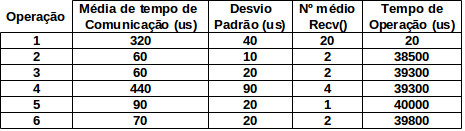
\includegraphics[width=\textwidth]{Imagens/t01.png}
%%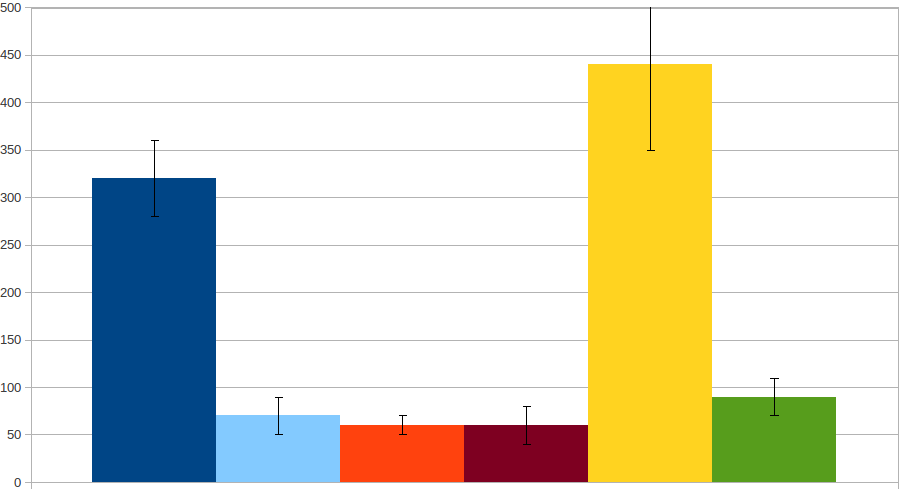
\includegraphics[width=\textwidth]{Imagens/g01.png}
%%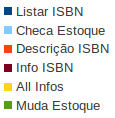
\includegraphics{Imagens/g011.png}
\caption{Gráfico Operação x Tempo Médio de Comunicação}
\end{figure}

Da tabela, percebe-se que os tempos de envio de um datagrama são basicamente o mesmo. Entretantos, também é possível perceber uma diferença muito grande nos tempos de envio para as operações de List e de All Information, sendo que o tempo desta última é quase o dobro do tempo da primeira. Elas são de longe as operações mais custosas realizadas quando analisamos os tempos de transmissão, apesar de não necessariamente serem as mais custosas quando o enfoque é o tempo de operação.
	
	Como previsto, a operação mais custosa é também a que envia a maior quantidade de dados. De fato, All Information envia todos os dados que estão no banco de dados, então é de se esperar que ela envie uma quantidade de dados sempre muito maior do que a enviada por qualquer outra operação. Isso fez com que seu tempo de envio fosse maior do que a soma de todos os outros tempos de envio!
	
	Sob esse mesmo raciocínio, seria estranho, então, a operação List ser a segunda mais custosa, já que na realidade, ela pode não enviar uma quantidade tão grande assim de dados. Na realidade, no caso do banco de dados utilizados para esse projeto, a quantidade de dados enviados pela operação List não passou de 1200 bytes.
	
	Considere como exemplo o livro Dom Casmurro – ISBN 9878765654, cuja operação de envio de descrição enviaria 2010 bytes, um pouco menos do que o dobro do enviado pela List. Entretanto, o tempo médio gasto com essa é mais do que 10 vezes o tempo médio do envio de uma descrição.
	
	Esse aparente erro é explicado quando considera-se o segundo fator apontado! Da tabela vemos que a implementação do servidor faz com que a média de chamadas de \textit{recvfrom} por parte do cliente seja de 33 (2 a mais do que na operação All Information). Essa quantidade é enorme quando comparada com as das outras operações. O servidor acaba por quebrar os dados em vários datagramas, e envia-os através de várias chamadas. Isso explica então o tempo de envio absurdo da operação List comprovando que quando se deseja determinar o tempo de transmissão de um dado, tão importante quanto determinar o tamanho da mensagem é determinar como essa mensagem será enviada!
	

	Por fim, montou-se um gráfico com essa tabela e seus desvios padrão:
	
\begin{figure}[h!]
%\caption{Dados da Transmissão em todas as operações numa mesma Máquina}
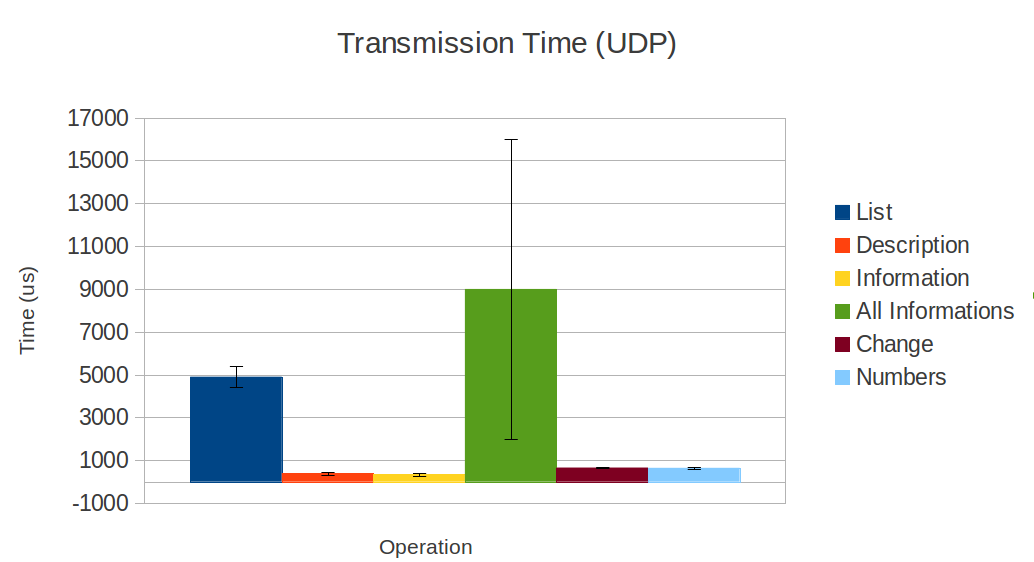
\includegraphics[width=\textwidth]{Imagens/udp.png}
%%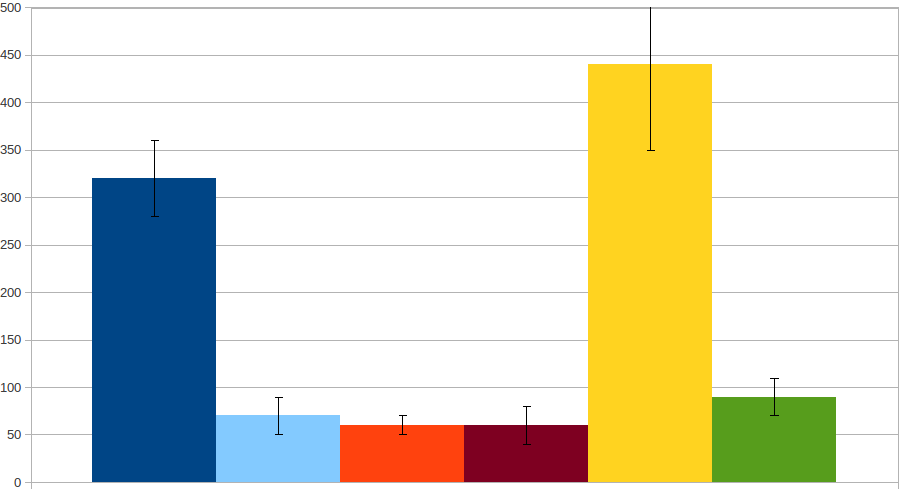
\includegraphics[width=\textwidth]{Imagens/g01.png}
%%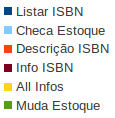
\includegraphics{Imagens/g011.png}
\caption{Gráfico Operação x Tempo Médio de Comunicação}
\end{figure}
	
	Note que o desvio padrão envolvido com cada medição é maior conforme o tempo da medição é maior. Isso também é natural do comportamento UDP, já que os tempos de operação podem variar muito devido a ser um protocolo não orientado a conexão.
	
\newpage
\section{Comparando UDP e TCP}
Para fazer uma comparação boa entre os dois protocolos, da mesma forma que no UDP, foram feitas uma série de medidas. Para o caso do TCP foram coletadas no mínimo 100 medidas, todas realizadas nas mesmas máquinas que as utilizadas no UDP.
	Com os dados, foi montada a seguinte tabela, que segue o formato da Tabela 01:
	
	%%%%% TABELA 2x
	
	\begin{table}[h]
\caption{Tabela Final TCP}
\begin{tabular}{|c|c|c|c|c|c|c|}
\hline 
Operação & Transmissão (us) & Erro (us) & Receives (us) & Erros (us) & Tempo de Opeação (us) & Erro (us) \\ 
\hline 
List & 5300 & 300 & 3 & 0 & 400 & 30 \\ 
\hline 
Description & 600 & 100 & 2 & 0.06 & 48100 & 700 \\ 
\hline 
Information & 500 & 100 & 2 & 0.07 & 49000 & 6000 \\ 
\hline 
All Informations & 4200 & 500 & 6 & 0.9 & 700 & 100 \\ 
\hline 
Change & 630 & 40 & 1 & 0 & 49000 & 9000 \\ 
\hline 
Numbers & 700 & 200 & 2 & 0.07 & 45000 & 2000 \\ 
\hline 
\end{tabular} 
\caption{Dados da Transmissão entre dois computadores por protocolo TCP}
\end{table}
	
	Para uma maior facilidade na comparação, a Tabela 01 é mostrada abaixo:
	
	%%%%% TABELA 3
\begin{table}[h]
\caption{Tabela Final UDP}
\begin{tabular}{|c|c|c|c|c|c|c|}
\hline 
Operação & Transmissão (us) & Erro (us) & Receives (us) & Erros (us) & Tempo de Opeação (us) & Erro (us) \\ 
\hline 
List & 4900 & 500 & 33 & 0 & 400 & 100 \\ 
\hline 
Description & 400 & 70 & 2 & 0 & 7900 & 500 \\ 
\hline 
Information & 350 & 70 & 2 & 0 & 8000 & 4000 \\ 
\hline 
All Informations & 9000 & 7000 & 31 & 0 & 800 & 200 \\ 
\hline 
Change & 660 & 40 & 1 & 0 & 50000 & 1000 \\ 
\hline 
Numbers & 650 & 50 & 2 & 0 & 4000 & 600 \\ 
\hline 
\end{tabular}
\caption{Dados da Transmissão entre dois computadores por protocolo UDP}
\end{table}
Observa-se que para os tempos de envio, o protocolo UDP mostrou-se mais rápido em quase todas as operações.

	Entretanto, os tempos do UDP não se mostraram tão satisfatórios assim quando comparam-se 3 operações (List, All Informations e Change) sendo que para as duas últimas os tempos foram na realidade maiores, apesar de que se considerarmos os erros envolvidos, na realidade todas estão aceitaveis, pois são cobertas pelos erros.
	
	Como considerou-se o mesmo banco de dados, os dados a serem enviados tinham o mesmo tamanho, logo esse não pode ser um fator tão importante para o envio.
	
	Novamente, a resposta está no segundo fator de atraso: a quantidade de mensagens enviadas! Podemos ver que para o caso de List, o UDP enviou cerca de onze vezes mais mensagens enquanto que para All Informations, esse numero foi de aproximadamente 5,2 vezes. Apesar disso, essa explicação não pode ser usada para justificar a operação Change, que no final das contas teve um desempenho pior no UDP.

	Uma observação final deve ser feita ainda. No caso especial da operação List, é notável que o UDP seja muito mais rápido, mesmo enviando uma quantidade tão grande de mensagens quando comparadas com número de mensagens enviadas pelo protocolo TCP. Atribuimos esse grande atraso do TCP as operações que tornam o protocolo confiavel, ou seja, a checagem de erros e ordem que o protocolo executa sempre que envia mensagens.
	
\begin{figure}[h!]
%\caption{Dados da Transmissão em todas as operações numa mesma Máquina}
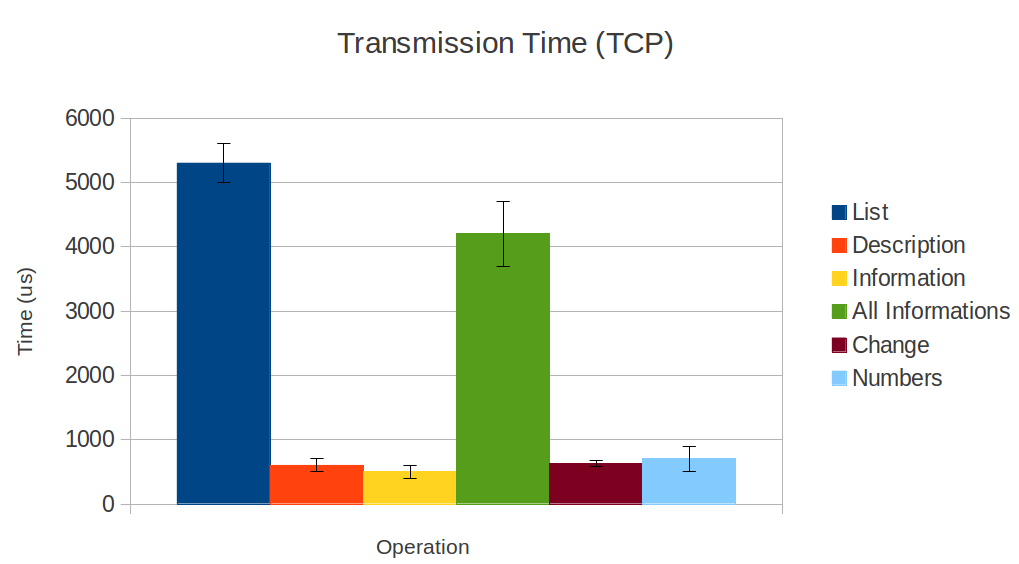
\includegraphics[width=\textwidth]{Imagens/tcp.png}
%%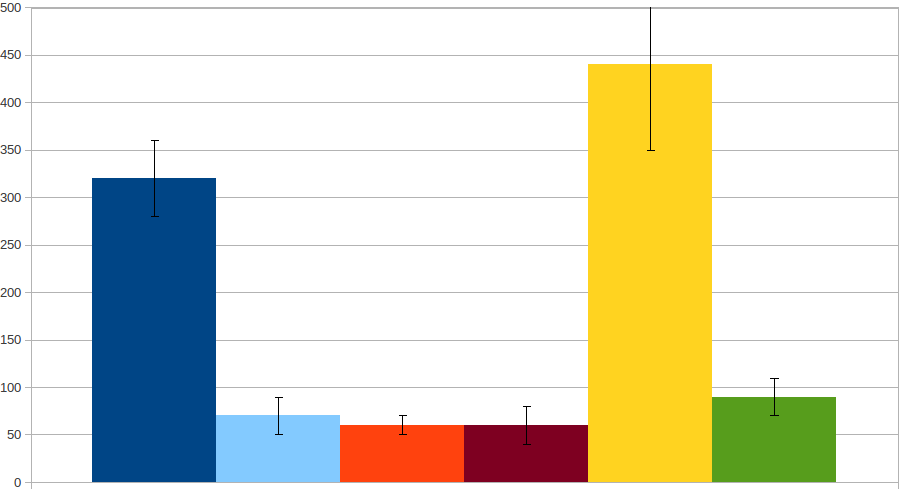
\includegraphics[width=\textwidth]{Imagens/g01.png}
%%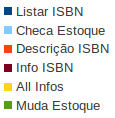
\includegraphics{Imagens/g011.png}
\caption{Gráfico Operação x Tempo Médio de Comunicação}
\end{figure}
	
\chapter{Conclusão}
Assim como observado para o protocolo TCP, pudemos determinar aqui os fatores que importam quando consideramos o protocolo UDP.

	Assim como no TCP, o UDP tem dois fatores principais. O primeiro e mais óbvio, é o tamanho e quantidade de dados que será enviado pelo protocolo. Vimos que no caso do UDP, esse foi o fator determinante para as medições de tempo, ao contrário do que aconteceu no caso do TCP. Isso era o esperado, pois o UDP não é um protocolo confiavel, logo ele simplesmente envia o que foi pedido para ser enviado, sem se preocupar com qualquer tipo de erro no envio.

	Entretanto, nunca poderemos desconsiderar a quantidade de mensagens enviadas para termos a transmissão do dado. Mesmo não sendo confiavel, pela Tabela 01, pode-se observar que o tempo de envio de uma operação é fortemente influenciado pela quantidade de mensagens envolvidas nessa transmissao.

	Ao final do projeto, percebe-se aqui as grandes diferenças que um protocolo confiavel e orientado a conexão (TCP) possui de um protocolo que prioriza a velocidade (UDP). De fato, o UDP provou-se mais rápido em todas as situações, se considerarmos a quantidade de mensagens enviadas. Isso explica porque ele é usado por aplicações que necessitam de grandes velocidades.

	De fato, essa velocidade deve ser sempre considerada, mesmo em casos onde faz-se necessario a confiabilidade. Para tais casos, o UDP pode ser utilizado, valendo-se o esforço em nível de aplicação para garantir-se a confiabilidade! Exemplo de aplicação assim é o DNS.

\chapter{Referências Bibliográficas}
"Beej's Guide to Network Programming". <http://beej.us/guide/bgnet/>. (Acesso em: 04 abril 2013). \\
"SQLite Documents". <http://www.sqlite.org/docs.html>. (Acesso em: 03 abril 2013).

\end{document}